\chapter{Deep Learning}
\label{ch:deep_learning}

\subsection{Biological Neuron}
The human nervous system is the largest information processor in the human body. It is not the only information processor, but it is the largest and most efficient one. The human nervous system consists of several components. First, the brain, which is responsible for processing information and making decisions. Information to the brain comes from the senses along nerve fibers. The brain processes this information and decides how to react in a given situation. This solution is transmitted along the nerve fibers in the opposite direction to the muscles. This is how information is processed in the human body. The nervous system has several components. These components are responsible for different tasks. However, all of these components are made up of roughly the same cells called neurons.

A neuron is a component that makes up the entire human nervous system. Almost all neurons are structured roughly the same. 
So, a neuron has a neuron nucleus, which is also called the neuron body. An electrical charge is accumulated in the body of a neuron. From the body of the neuron there are many processes: there are small processes and large processes. The little outgrowths are so called dendrites. Through these processes, a signal from other neurons comes to our neuron. There is a large scion. This process is called an axon. A neuron transmits a signal to other neurons along the axon. The place where the axon of another neuron connects to the dendrites of our neuron is called a "synapse". The synapse is where the dendrite and axon meet. A synapse can be strong or it can be weak. If the synapse is strong, then the signal that is transmitted along the axon of the neuron will almost completely go to our neuron. If the synapse is weak, then practically no charge will cross from the axon of another neuron to our neuron. The synapse can change over time. Depending on the circumstances, the synapse can get stronger or it can get weaker. It is with the synapse tuning that the training of the biological neural network and, accordingly, the human nervous system is connected.

Considered visualization of the described above processes is as follows:
\begin{figure}[h]
    \centering 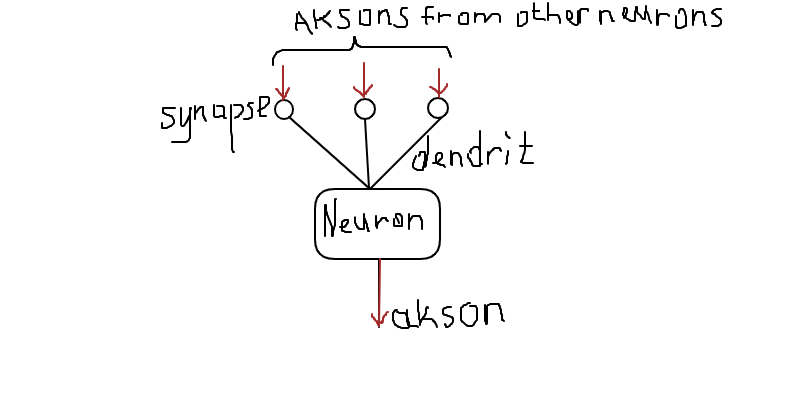
\includegraphics[width=7cm]{images/neuron_biological_model.png}
    \caption {biological model of neuron}
\end{figure}    

\subsection{Neuron mathematical model}
Initially for simplicity we will represent neuron mathematical model graphically. It should be taken into consideration, the red characters denote tune parameters of the neuron.     
\begin{figure}[h]
    \centering 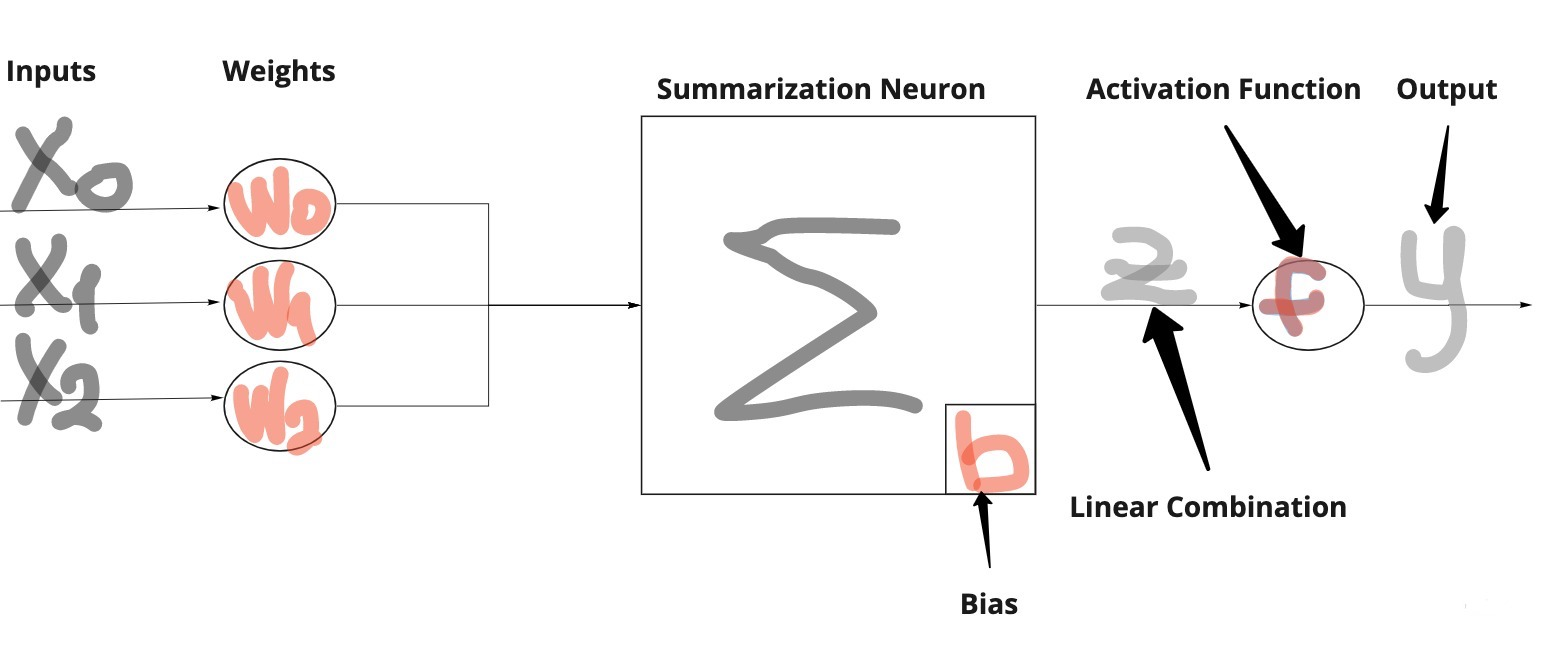
\includegraphics[width=7cm]{images/neuron_math_model.jpg}
    \caption {mathematical model of neuron}
\end{figure} 

In the mathematical model of the neuron, the body of the neuron, where the input signals accumulates, is replaced by a summarizing neuron. In addition, the biological neuron also has axons and dendrites, which get the inputs and send the outputs. Accordingly, in our mathematical model of the neuron, we will add inputs and outputs to the summarizing neuron. It's also worth keep in mind the biological neuron applies some actions with the signals that come into it, namely, it accumulates charge until it reaches some point and only after that forwards it further. This is what we will do in the mathematical model of the neuron using the activation functions.

Afterwards, model of neuron can be mathematically defined as:
\[ y = f(z) = f(w_0*x_0+w_1*x_1+w_2*x_2+b) = f(\sum\limits_{i=0}^{N-1} w_i*x_i+b) = f(<\overrightarrow{w}, \overrightarrow{x}>+b) \]
Where:
\begin{itemize}
    \item $x_0, x_1, x_2$: inputs
    \item $w_0, w_1, w_2$: input weights 
    \item $b$: some bias for increasing non-linearity   
    \item $f(z)$: some activation function 
\end{itemize}

\subsection{Activation function}




